\documentclass[letterpaper]{article}

%pass the page height/width into pdflatex, otherwise it assumes A4
\pdfpagewidth=\paperwidth
\pdfpageheight=\paperheight

\usepackage{graphicx} %get graphics commands
\usepackage{times}

%get \FloatBarrier command
\usepackage{placeins} 

%give option to use commands like 0.5\textwidth for distances
\usepackage{calc} 
 %allows wraping figures around text
\usepackage{wrapfig}

%adds option to include verbatim input from files
\usepackage{moreverb} 

%Set the pages margins to 1 inch, all the way around
\usepackage{anysize}
\marginsize{1in}{1in}{0.45in}{0.45in}

\begin{document}

\begin{figure}[htbp]
\begin{center}
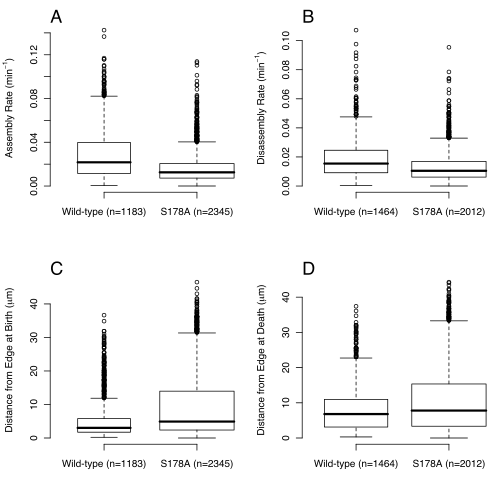
\includegraphics{../figures/unfilt_S178A_vs_wild-type}
\caption{default}
\label{default}
\end{center}
\end{figure}

\end{document}